\chapter{绪论} 
\thispagestyle{others} 
\pagestyle{others} 
\xiaosi 

\section{研究背景及意义}
随着大数据时代和人工智能技术的迅猛发展,数据资源已成为驱动各行各业决策能力和服务质量提升的重要战略要素。然而,数据隐私保护法规日益严格,以及广泛存在的数据孤岛现象,使得不同机构之间的数据协作面临着前所未有的挑战,严重制约了数据价值的充分挖掘。在此背景下,联邦学习\textsuperscript{\cite{chen2021secureboost+,de2010practical}}作为一种新兴的分布式机器学习方法应运而生,通过允许多个数据拥有方在不共享原始数据的基础上,通过交换模型参数或梯度信息实现模型联合训练,成功解决了数据隐私保护与联合建模之间的矛盾。在联邦学习的众多研究方向中,纵向联邦学习(Vertical Federated Learning,VFL)因其能够有效整合不同机构所拥有的互补特征数据而得到广泛关注,并被广泛应用于金融、医疗、推荐系统等领域。然而,目前联邦学习主要集中于监督学习领域,严重依赖大量的标记和对齐数据,但实际应用场景中却普遍面临标注成本高、领域专家稀缺、资源受限以及样本对齐不足等现实挑战,导致大量潜在有用数据无法被有效利用,进而制约了模型泛化能力与应用效果的提升\textsuperscript{\cite{li2021comatch}}。此外,在现实应用中常常只有一方拥有标签信息,这进一步加剧了联合模型训练的复杂性和挑战。因此,如何高效利用未完全标记数据和未对齐样本成为当前纵向联邦学习领域亟待解决的重要课题。

针对上述问题,本研究提出了一种融合纵向联邦学习与半监督PU学习技术的方法(Vertical Federated learning with Positive and Unlabeled data,VFPU),有效地解决了未标记数据缺失的PU学习(Unlabeled-Data-Deficient PU,UDD-PU)问题。此外,本研究进一步提出一种基于纵向联邦半监督学习的样本生成方法(Participants Sample Generation method based on VFPU-Multitask,FedPSG-PUM),通过融合半监督学习与数据生成技术,在不共享原始数据和模型参数的前提下,实现对未对齐样本的高效利用。具体而言,VFPU方法允许多方在保护数据隐私的基础上,通过交换加密后的中间计算结果实现联合模型训练,有效弥补了现有联邦学习框架处理未完全标记数据的不足,拓宽了PU学习在真实业务场景中的应用范围。FedPSG-PUM方法则通过分析特征间相关性、伪标签预测和表格数据生成,有效解决了纵向联邦学习中样本对齐不足和标签信息缺失的难题,显著提高了数据资源的利用效率和模型的泛化性能。这些方法的提出不仅在理论上丰富了联邦学习与半监督学习的研究范畴,也为金融风险控制、医疗诊断预测、精准医疗、智能制造预测性维护和智能推荐系统等领域提供了切实可行的解决方案,有助于各行业在确保数据隐私安全的基础上更精准地进行数据驱动决策。这些研究成果不仅为联邦学习场景下复杂半监督学习问题提供了理论支撑和实践指导,也为未来的数据合作与价值共享提供了宝贵的技术路径与方法论支持。



\section{国内外研究现状}
\subsection{联邦半监督学习}
当前的联邦半监督学习方法大多基于横向联邦架构(Horizontal Federated Learning),在这种架构下,各参与方共享相同的特征空间,但其样本ID不同。具体来说,横向联邦学习允许多个客户端在不交换原始数据的前提下,通过交换模型参数或梯度来共同训练机器学习模型。在联邦半监督学习的应用中,根据标注数据的位置的不同,通常可以将其分为两种情况:一种是标签存储在客户端,即每个参与方仅拥有自己数据的标注信息;另一种情况是标签存储在服务器端,在这种情况下,服务器负责汇总所有标注信息并协调各参与方的学习过程。这两种情况在实际应用中各有优劣,涉及的技术细节和隐私保护策略也有所不同。随着越来越多的应用场景对数据隐私的要求日益严格,如何有效地进行半监督学习,特别是在横向联邦学习框架下,在确保数据隐私的同时提升模型性能,已成为当前研究的热点之一\textsuperscript{\cite{jin2023federated}}。

(1) 标签在客户端

标注数据存于客户端,而服务器只能获取未标注数据。例如,某家公司欲利用智能手机拍摄的图片训练一个物体检测的联邦学习模型,但无法直接访问用户的本地数据,只能依赖用户的标注,如图 \ref{LabelAtClient} 所示。首先,对于不同的参与方(用户),样本ID是不同的,但参与方(用户)手机里的图片特征是一样的,所以构成了横向联邦的设置。其次,用户通常不愿为每张照片标注,给基于横向联邦的半监督学习创造了一个“客户端标注”(label-at-client)的环境。

\vspace{-0.1cm}
\begin{figure}[h]
	\centering
	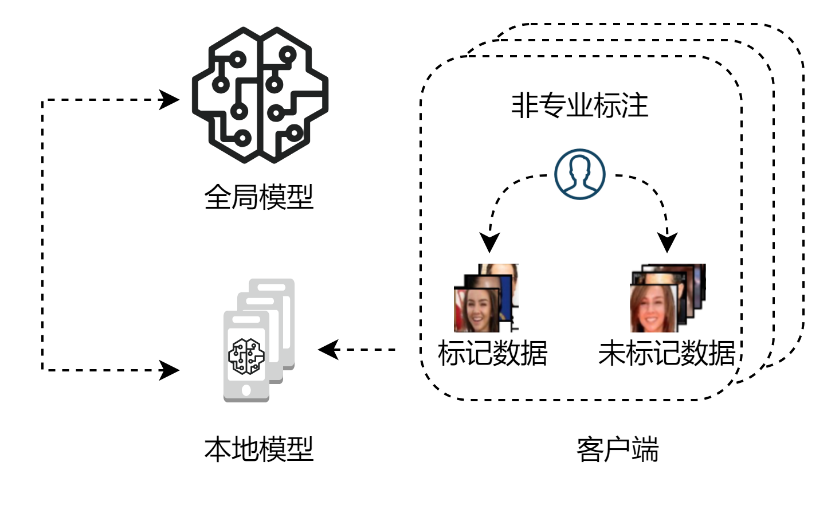
\includegraphics[width=10cm]{chapters/imgs/LabelAtClient}
	\bicaption[\xiaosi 标记数据在客户端的情况]
	{\wuhao 标记数据在客户端的情况}
	{\wuhao Labeled data on the client side}
	\label{LabelAtClient}
\end{figure}
\vspace{-0.35cm}

RSCFed\textsuperscript{\cite{liang2022rscfed}} 主要关注联邦半监督学习中的标签隔离问题和数据异质性问题。在局部训练中,采用师生模型\textsuperscript{\cite{tarvainen2017mean}}对无标签数据进行训练。为进一步解决数据异质性问题,RSCFed 提出了子共识抽样法和距离加权聚合法。在每一轮中,通过对所有参与者的多个子集进行独立抽样,从而聚合出多个子共识模型,这样每个子共识模型都有望包含拥有标记数据的参与者。此外,本地模型会根据它们与子共识模型的距离进行加权,这样偏差模型就会得到较低的权重,其影响也会降到最低。

FedSSL\textsuperscript{\cite{fan2022private}}解决了标签隔离问题、数据隐私问题和数据异构问题。为了便于对未标记的客户端进行本地训练,FedSSL利用了伪标记技术。此外,为解决数据异构问题,FedSSL学习全局生成模型,从统一的特征空间生成数据,从而通过生成的数据缓解数据异构问题。最后,为了防止生成模型造成的隐私泄露,FedSSL利用差分隐私(DP)来限制生成模型中训练数据的信息泄露。

FedMatch\textsuperscript{\cite{jeong2020federated}}提出了一种客户端间一致性损失来解决数据异质性问题。具体来说,对每个客户端的前k个最近客户端进行采样,在每个数据样本上,本这样,每个客户端只负责学习正类,并可自行进行局部训练。根据经验,在正类和无标签学习设置中,所提出的FedPU优于FedMatch。


AdaFedSemi\textsuperscript{\cite{wang2022enhancing}}提出了一种系统,可在联合半监督学习中利用服务器端无标记数据实现效率与模型准确性之间的权衡。在每一轮学习中,模型都是通过客户端的标注数据进行训练,并在服务器端进行汇总。服务器端未标注数据通过伪标注纳入训练过程。AdaFedSemi确定了平衡效率和性能的两个关键参数,即客户端参与率P和伪标签的置信度阈值τ。较低的P可以降低通信成本和模型准确性,而较高的τ可以降低服务器端计算成本,同时也限制了未标记数据的使用。实验表明,AdaFedSemi通过动态调整P和τ在不同的训练阶段实现了效率和准确性之间的良好平衡。


DS-FL\textsuperscript{\cite{itahara2021distillation}}解决了与AdaFedSemi类似的问题,即客户端拥有标签数据,而服务器拥有非标签数据。它提出了一种集合伪标签解决方案来利用服务器端的非标签数据。具体来说,它不是对数据样本使用单一的伪标签,而是对所有客户端生成的伪标签进行平均。这将创建一个客户端模型集合,并提供更好的性能。

(2) 标签在服务器端

标注数据存于服务器,而客户端只有未标注数据。例如,一家可穿戴设备公司希望利用联邦学习训练健康监测模型,如图 \ref{LabelAtServer} 所示。在这种情况下,由于用户通常缺乏专业知识,无法标注健康相关数据,因此客户端的数据是未标注的。标签数据在客户端的情况比标签在服务器端设置更复杂,原因是所有客户端都只拥有未标记数据,无法为联邦模型提供额外的监督信号,仅使用无标签数据进行训练可能会导致遗忘从有标签数据中学到的知识,从而影响模型性能\textsuperscript{\cite{jeong2020federated,diao2022semifl}}。

%\vspace{-0.1cm}
\begin{figure}[H]
	\centering
	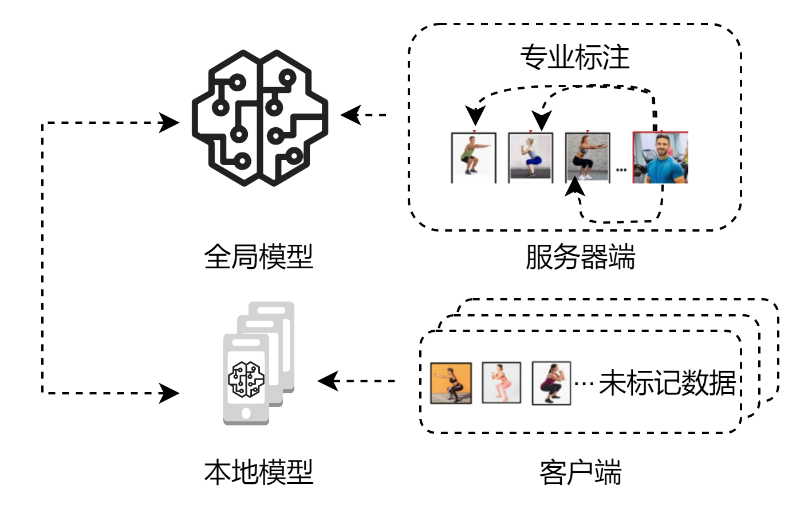
\includegraphics[width=10cm]{chapters/imgs/LabelAtServer}
	\bicaption[\xiaosi 标记数据在服务端的情况]
	{\wuhao 标记数据在服务端的情况}
	{\wuhao Labeled data on the server side}
	\label{LabelAtServer}
\end{figure}
\vspace{-0.35cm}

为了解决标签数据和非标签数据之间的隔离问题,FedMatch\textsuperscript{\cite{jeong2020federated}}提出了一种不相干的学习方案,即分别为标签数据和非标签数据设置两套参数。在非标签数据上进行训练时,标签数据的参数是固定的,反之亦然,以防止知识被覆盖。非标记数据的参数会在参与者和服务器之间传输,而非标记数据的参数设置为稀疏的,这为通信效率带来了额外的好处。此外,为了解决不同客户端持有的异构数据问题,FedMatch 提出了客户端间一致性损失,这样不同参与者的本地模型就能在相同数据上产生相似的输出。

%\vspace{-0.5cm}
\begin{table}[h]
	\centering
	\bicaption[\xiaosi \songti 联邦半监督学习方法总结]
	{\songti \wuhao 联邦半监督学习方法总结}
	{\songti \wuhao Summary of federated semi-supervised learning methods}
	\label{SummaryOfFedSemi}
	\resizebox{\textwidth}{!}{
		{\songti \wuhao
			\begin{tabular}{cccccc}
				\toprule[1.5pt]
				类别 & 方法 & 半监督学习算法 & 隐私保护方案 & 数据异质问题 & 性能 \\
				\midrule
				\multirow{6}{*}{标签在客户端} 
				& RSCFed     & 教师学生模型 & 无     & 加权距离聚合   & 无                \\
				& FedSSL     & 伪标记       & 差分隐私 & 全局生成模型     & 无               \\
				& FedMatch   & 伪标记       & 无     & 客户端间一致性  & 分散学习和稀疏学习 \\
				& FedPU      & PU Learning  & 无     & 客户端间一致性  & 无                \\
				& AdaFedSemi & 伪标记       & 无     & 无             & 调整置信度阈值和参与率 \\
				& DS-FL      & 集成未标记   & 无     & 无             & 传输日志、无参数     \\
				\midrule
				\multirow{2}{*}{标签在服务器端} 
				& SemiFL     & 伪标记       & 无     & 减少熵的平均值   &                   \\
				& FedMatch   & 伪标记       & 无     & 客户端间一致性   & 分散学习和稀疏学习   \\
				\bottomrule[1.5pt]
			\end{tabular}
		}
	}
\end{table}
\vspace{-0.35cm}

SemiFL\textsuperscript{\cite{diao2022semifl}}采用另一种方法来解决这些挑战。它建议使用标注数据对全局模型进行微调,以提高其质量,并减轻客户端无监督训练所造成的遗忘。此外,SemiFL建议最大限度地提高客户端模型与全局模型之间的一致性,而不是在客户端之间对模型输出进行正则化。具体来说,全局模型为客户端的未标记数据生成伪标签,而客户端的局部模型则根据伪标签进行训练。实证结果表明,与FedMatch相比,SemiFL能产生更有竞争力的结果。

(3) 联邦半监督学习方法总结

表 \ref{SummaryOfFedSemi} 总结了前文介绍的基于横向联邦的半监督学习方法,按照标签在客户端或服务器端进行划分。从表中可以看出,这些方法在半监督学习算法、隐私保护方案、数据异质问题和性能提升策略方面存在着较大差异。当标签位于客户端时,这些方法主要采用教师学生模型、伪标记和PU学习等半监督学习算法,其中FedSSL方法通过差分隐私来保护数据隐私,FedMatch则强调客户端间的一致性,AdaFedSemi则通过调整置信度阈值和客户端参与率来提高模型性能。



\subsection{数据生成方法}
生成合成数据的主要策略集中在生成模型上,这些模型旨在从现有数据集中学习丰富的表示,并随后生成新的样本。这些方法在多个领域中得到了应用,如医学研究、金融、教育以及各种工业应用,其中高质量合成数据的生成对于隐私保护和有限数据集的增强都至关重要。以下将对常见的数据生成方法进行详细介绍。

基于自编码器的方法:这一类别中的先驱性工作是自编码器(Autoencoder,AE)\textsuperscript{\cite{hinton2006reducing}},其训练目的是将高维输入映射到低维潜在编码中,然后从这些编码中重构原始数据。通过强制隐藏(潜在)层降维,AE有效地学习到了压缩表示。然而,纯粹的AE是确定性的,缺乏灵活采样的直接机制。变分自编码器(Variational Autoencoder,VAE)\textsuperscript{\cite{kingma2013auto}} 通过引入概率潜在变量框架解决了这一问题,从而可以从学习到的潜在分布中采样出新的、未见过的数据点。这一扩展极大地拓宽了基于自编码器模型在合成数据生成中的潜在应用范围。在AE和VAE的基础上,Xu等人\textsuperscript{\cite{xu2019modeling}} 提出了一种针对表格数据生成和重构的改进方法。其方法更准确地建模了潜在变量与表格特征的联合分布,而后者可能包含连续和离散属性。通过关注不同类型变量之间的相互作用,该方法确保生成的合成数据忠实地反映了真实世界表格数据集(如医疗和教育数据)中存在的复杂依赖关系。

基于生成对抗网络(Generative Adversarial Networks,GANs)\textsuperscript{\cite{goodfellow2014generative}}的方法:自2014年引入以来,GANs对生成建模领域产生了重大影响。其基本概念基于博弈论:两个网络——生成器(Generator,G)和判别器(Discriminator,D)——在对抗循环中训练。判别器学习区分真实数据和合成数据,而生成器则试图生成能够欺骗判别器的样本。当判别器无法再区分真实数据与生成数据时,这个极小极大博弈就告一段落,这表明生成器已经捕捉到了底层分布的统计特征。在GANs出现后不久,\textsuperscript{\cite{mirza2014conditional}} 提出了条件生成对抗网络(Conditional Generative Adversarial Networks,CGANs),其中生成器和判别器均基于辅助信息(如类别标签或特定输入变量)进行条件化。这一扩展框架使得生成能够针对特定类别或属性进行定向,实际上将原本的无监督设置转变为有监督或半监督范式。尽管取得了这些进展,传统GANs往往仍然面临梯度消失或模式崩溃的问题。为了解决这些问题,Banach等人用Wasserstein距离替换了Jensen–Shannon(JS)和Kullback–Leibler(KL)散度,从而诞生了Wasserstein GAN(WGAN)\textsuperscript{\cite{adler2018banach,arjovsky2017towards}}。

针对表格数据的GANs:虽然GANs最初因图像合成而受到欢迎,但它们在处理通常具有异构特征类型、不平衡和复杂依赖关系的表格数据集时,同样证明既具有挑战性又极具价值。针对这些挑战,\textsuperscript{\cite{xu2018synthesizing}} 提出了表格GAN(Table GAN,TGAN),该方法在生成器网络中应用了长短期记忆单元,并在判别器中采用了多层感知器,从而使深度架构适应于表格数据生成(例如健康记录或学生成绩数据)。2019年,Xu、Lei等人\textsuperscript{\cite{xu2019modeling}}提出了CTGAN(Conditional Table GAN),一种专门为处理不平衡离散列、多模态连续列以及表格数据固有复杂性而设计的改进型条件GAN架构。

通过利用条件采样策略,CTGAN在建模详细分布和生成与真实数据密切对应的表格行方面表现出色。表格GANs的进一步发展,Lee等人\textsuperscript{\cite{lee2021invertible}}探索了一种可逆的表格GAN框架,该框架将对抗训练与来自可逆神经网络的负对数密度正则化相结合。该方法在训练过程中增加或降低真实样本的对数密度,从而根据隐私和质量目标生成更接近或更远离真实数据流形的合成样本。为了解决模式崩溃并提高样本多样性,Nguyen等人\textsuperscript{\cite{nguyen2017dual}}提出了一种双判别器GAN,该方法结合了KL散度和反向KL散度,以更好地捕捉真实世界数据分布的多模态特性。Singh等人\textsuperscript{\cite{singh2021metgan}} 针对内存限制问题提出了MeTGAN,在生成器和判别器中采用稀疏线性层,从而显著降低了内存开销,而对合成质量影响不大,这在处理具有高基数类别变量的表格数据集时尤为有利。在扩展CTGAN功能方面,Zhao等人\textsuperscript{\cite{zhao2021ctab}} 提出了CTAB-GAN,能够对连续、类别和混合类型的特征进行建模。该方法能够有效处理偏态分布和多样化的特征类型,通常在与真实数据的相似性和下游任务准确性方面优于其他基线方法。Engelmann最后,通过在真实数据集上的实验验证,系统评估所提方法的有效性和优越性,并分析其在隐私保护、数据异构性处理和性能优化方面的表现。

具体而言,本研究首先关注多方联邦环境下未标记数据的高效利用问题。在多方协作场景中,数据的异构性和隐私约束使得传统半监督学习方法难以直接适用。为此,本文在第3章提出了基于多方联邦的半监督学习方法VFPU,通过将PU学习技术适配到联邦学习框架中,设计了一种能够在有限标记数据条件下,利用多方未标记数据进行模型训练的算法。该方法在推荐系统等应用场景中表现出色,能够在保护数据隐私的同时,显著提升模型的精确率和召回率。

进一步地,本研究针对纵向联邦学习中对齐样本不足的问题,提出了FedPSG-PUM方法,并在第4章进行了详细阐述。FedPSG-PUM通过三个关键流程实现样本生成:一是计算跨方特征相关性,以识别参与方数据间的依赖关系;二是基于纵向联邦半监督学习预测未标记样本的伪标签,利用高相关性特征扩充训练数据;三是针对低相关性特征,引入生成模型合成数据,填补特征缺失,提升数据完整性。该方法不仅充分利用了对齐样本和非对齐样本,还通过隐私保护机制确保了数据安全,在小样本对齐场景下显著提高了模型的预测性能。

在实验验证方面,本研究选取了多个公开数据集,设计了一系列对比实验,分别评估VFPU和FedPSG-PUM在不同数据分布和样本对齐程度下的表现。实验结果表明,所提方法在性能上优于传统联邦学习和半监督学习基线方法,同时在隐私保护和计算效率上具有显著优势。此外,通过对算法参数和基础估计器的分析,进一步揭示了方法设计的合理性和优化空间,为后续研究提供了理论支持和实践指导。

总之,本论文通过将半监督学习与联邦学习相结合,提出了针对样本生成的新方法,解决了联邦学习中标记数据稀缺和样本对齐不足的关键问题。这些研究成果不仅丰富了联邦半监督学习领域的理论体系,还为医疗、金融、智能制造等需要隐私保护的分布式学习场景提供了可行解决方案,具有重要的学术价值和应用前景。

\section{论文组织结构}
为清晰呈现基于联邦半监督学习的样本生成方法的研究逻辑和内容体系,本文按照科学研究的惯例组织结构,共分为五章,各章内容安排紧扣研究主题,具有明确的层次性和递进性。以下对论文的组织结构进行详细阐述:

第一章为绪论部分。本章作为全文的开篇,系统梳理了研究的背景、意义及国内外研究现状,明确了联邦半监督学习和样本生成方法的研究热点与挑战。在此基础上,简要介绍了论文的主要研究内容,并通过本节对论文结构进行概述,为读者提供研究脉络的整体框架。通过对研究背景和现状的分析,本章旨在阐明研究的必要性与创新点,为后续章节的展开奠定基础。

第二章为相关理论介绍。本章详细阐述了本文研究所依赖的理论基础和关键技术。首先介绍了联邦学习的基本概念、分类及其在隐私保护中的应用;接着论述了半监督学习的核心思想、主要方法及其在数据稀缺场景下的优势;最后探讨了表格数据生成技术的原理与应用。通过对这些理论和方法的系统梳理,本章为后续提出的算法设计提供了坚实的理论支撑。

第三章为基于多方联邦的半监督学习方法研究。本章聚焦于多方联邦学习中未标记数据缺失的问题,提出了VFPU算法。首先分析了未标记数据缺失问题(UDD-PU)的定义与特性,随后详细介绍了VFPU算法的框架设计及其在多方联邦环境下的实现流程。通过在多个数据集上的实验验证,展示了VFPU在推荐任务中的优越性能,并对实验结果进行了深入分析,最后总结了本章的研究贡献与局限性。

第四章为基于半监督学习的纵向联邦参与方样本生成方法。本章针对纵向联邦学习中对齐样本不足的挑战,提出了FedPSG-PUM方法。本章首先分析了问题的定义与场景假设,随后系统阐述了FedPSG-PUM的整体框架,包括跨方特征相关性计算、半监督预测和生成模型合成三个核心流程,并对算法设计与实现细节进行了详细描述。通过多组实验验证了该方法在性能提升和隐私保护方面的有效性,并对结果进行了全面分析,最后总结了本章工作的创新点与应用价值。

第五章为总结与展望。本章对全文研究内容进行了归纳总结,提炼了基于联邦半监督学习的样本生成方法的核心成果与贡献,分析了所提方法的理论意义和实践价值。同时,针对研究中存在的不足之处,如算法在极端异构数据场景下的适应性以及计算复杂度的优化空间,提出了未来工作的改进方向和展望,为后续研究提供了参考。
\clearpage


